\chapter{Eredmények, konklúzió}

\section{Az első tesztek}

Először is az implementált modell helyességét kell megvizsgálni. Eh

\begin{figure}[H]
	\centering
	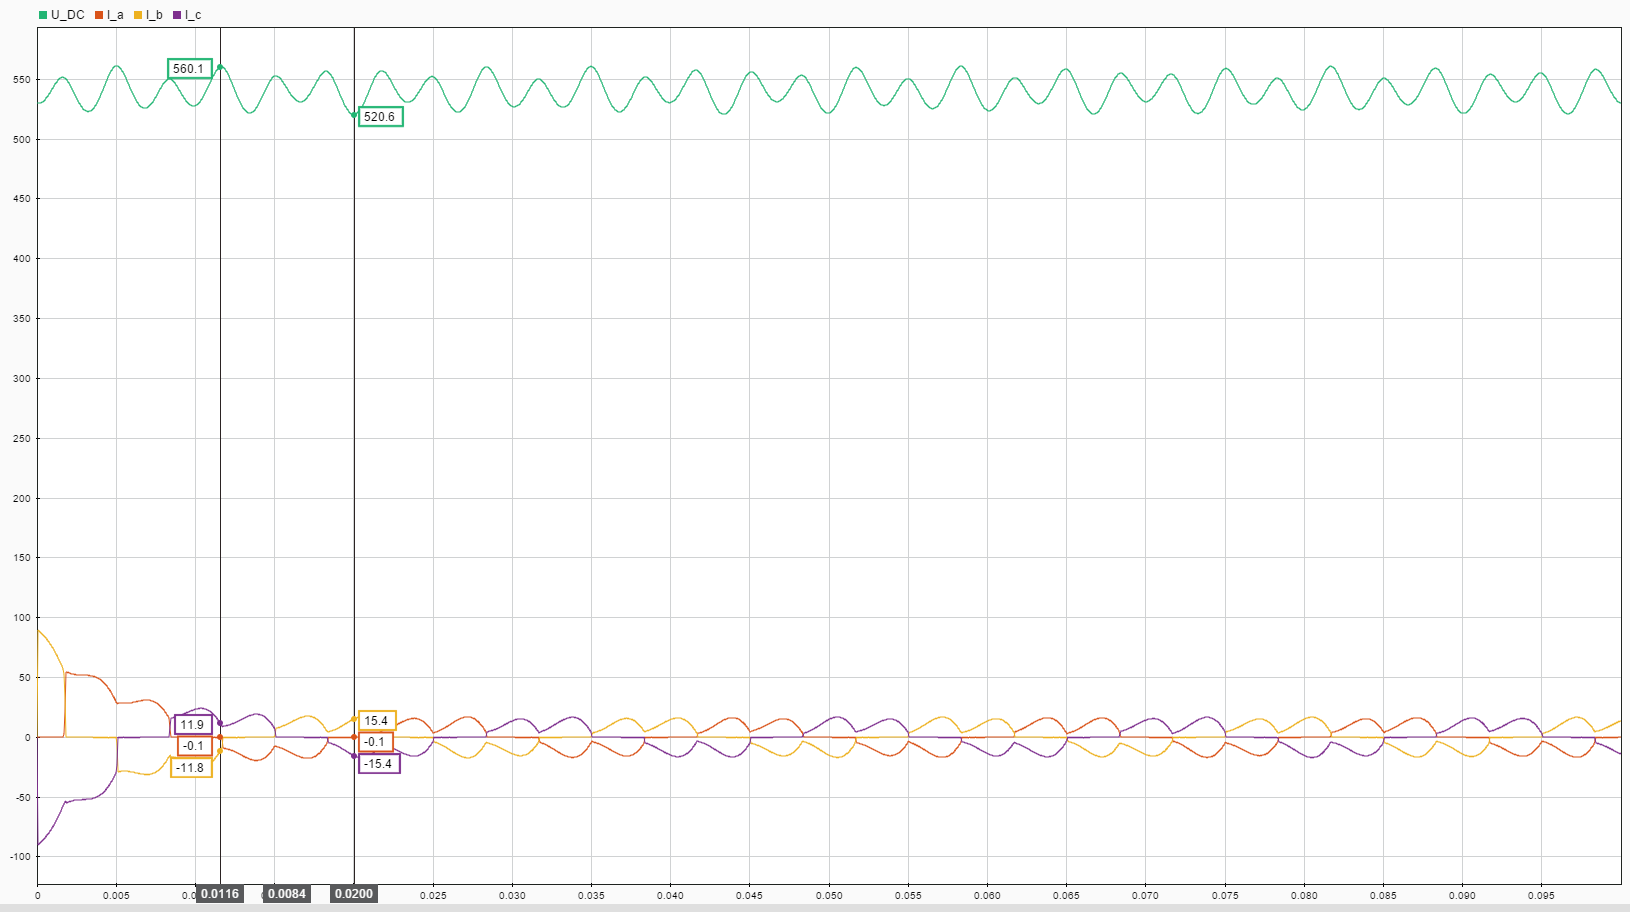
\includegraphics[width = \textwidth]{figures/continous_testrun_1.png}
	\caption{A szimuláció eredménye} 
	\label{fig:cont_run}
\end{figure}

\begin{figure}[H]
	\centering
	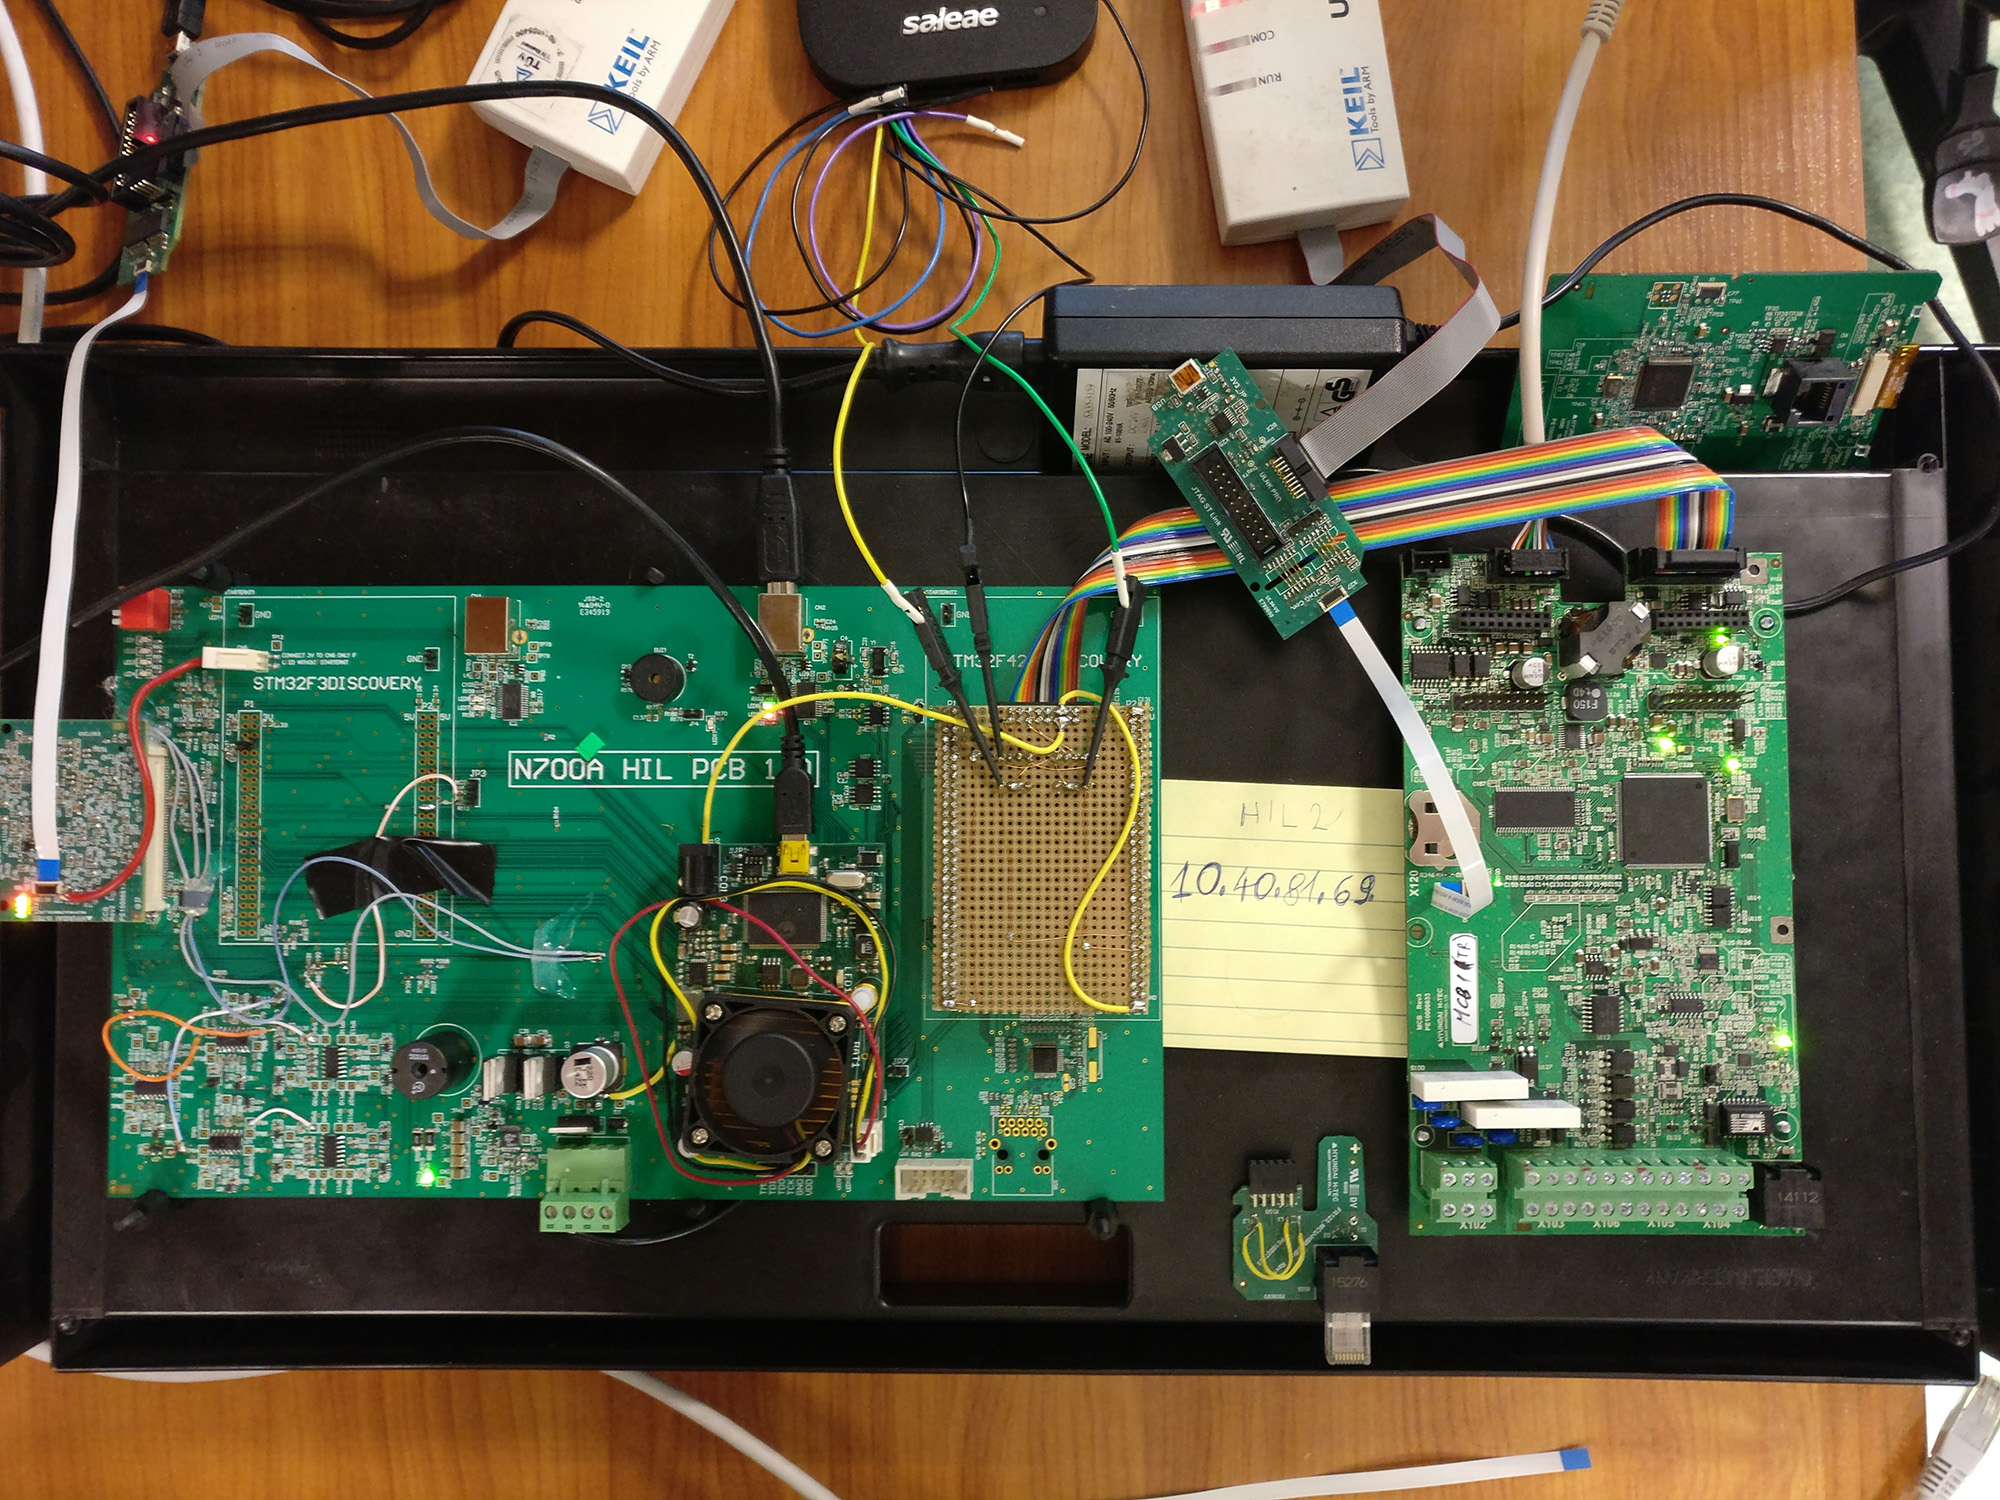
\includegraphics[width = \textwidth]{figures/hil_table.jpg}
	\caption{Az összeállított HIL deszkamodell} 
	\label{fig:hil_desk}
\end{figure}

\begin{figure}[H]
	\centering
	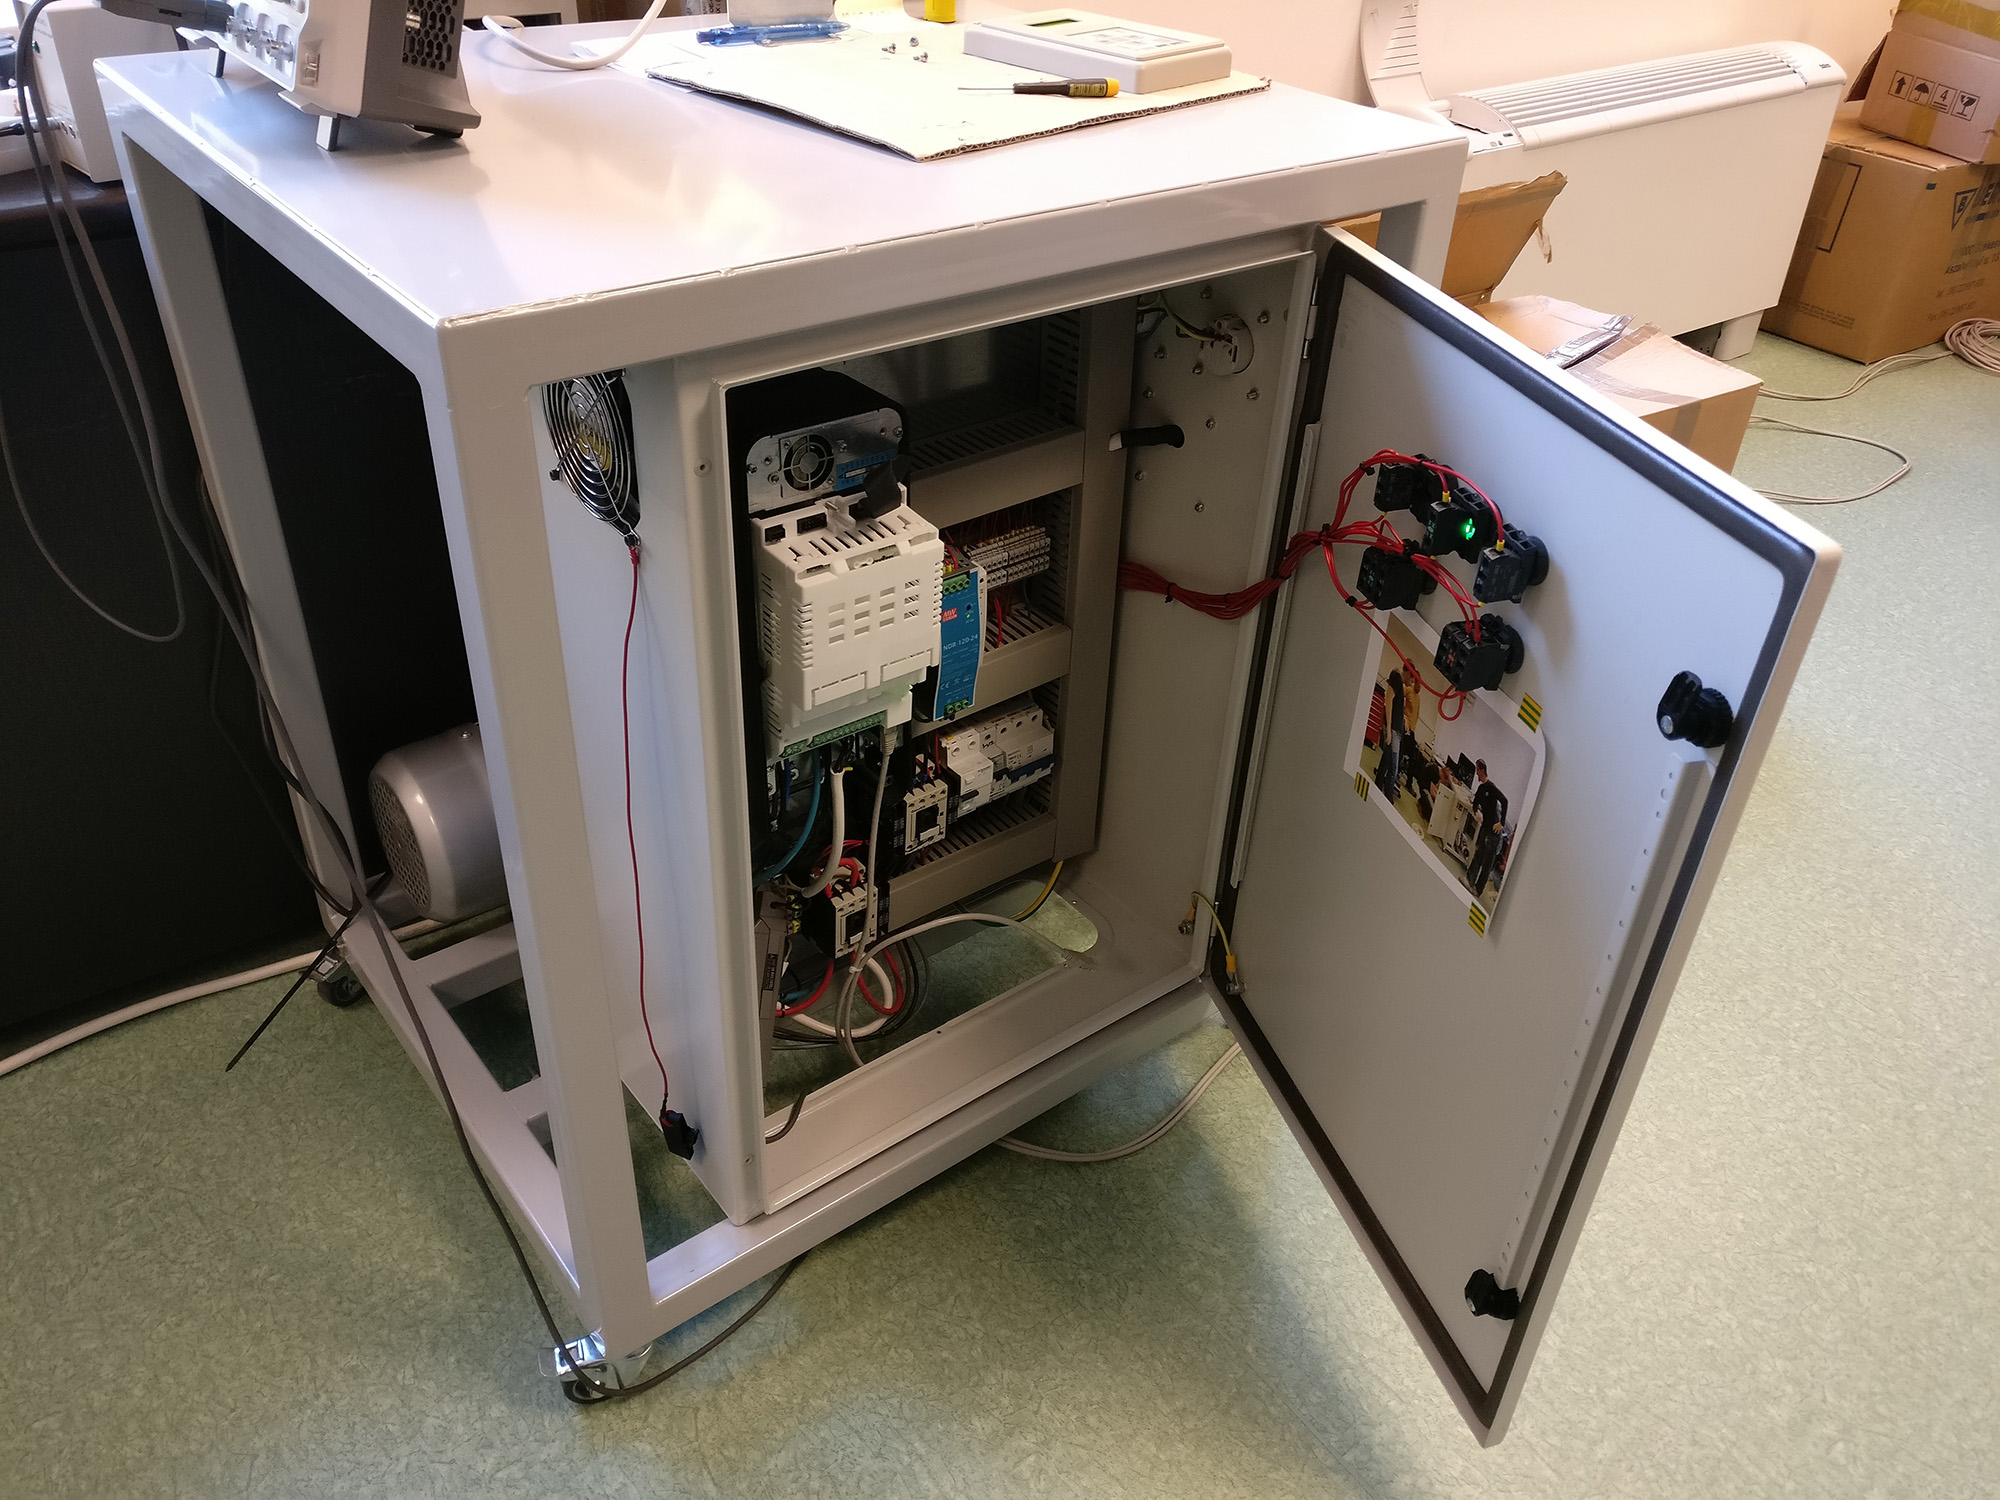
\includegraphics[width = \textwidth]{figures/office_testbench.jpg}
	\caption{Az ,,office testbench''} 
	\label{fig:office_testbench}
\end{figure}



\section{Konklúzió}

A dolgozat írása idején új hardware még nem készült el, a régin azonban el lettek végezve azoka a módosítások, melyek a jövőben gyártásba fognak kerülni. A jelenelg készített modellt így ki lehet próbálni, reprezentatív méréseket lehet rajta végezni.

A HIL-ben jelenleg a Frame 1 paraméterei szerinti modell található, ami jelen esetben különösen szerencsés, mert Frame 1-ből rendelkezésre áll egy laborban tesztelhető példány így a szimuláció közvetlenül összehasonlítható a valósággal.

\section{További lehetőségek}

Mint ahogy azt korábban is írtam, a téma még számos továbbfejlesztési lehetőséget tartogat magában. A bemeneti modellen lehet még fejleszteni ,hogy valóban minden lehetséges üzemállapotot szimulálni tudjunk. A jelenlegi konfiguráció a funkcionális tesztekhez elegendő, de még pontosabb teszteket tudunk végezni egy a valósághoz közelebb álló modellel.

Ezen felül látok még fejlődési lehetőséget magában a keretrendszerben is. A Vivado már támogat grafikus tervezést verilog szinten is, az egyes IP-k elérhetőek a Simulinkhez hasnló környezetben is, így a megfelelő összeköttetéseket grafikusan biztosítva. Termsézetesen a funkcionalitás leírását nem kerülhetjük el, azonban egy jobban áttekinthető és könnyebben szerkeszthető rendszert kapunk ilyen módon. Azt szeretném elérni ,hogy a MATLAB által generált modul elérhető legyen ilyen formában is, felgyorsítva ezzel a fejlesztést.